\chapter{Data acquisition for CHIPS}
\label{chap:daq}


\section{Things to talk about}


\section{Diagrams}

- Madison Diagrams
- Nikhef Diagrams
- Hut Diagrams
- Jelly box Diagrams
- Electronics box Diagrams
- Manifold diagram, with electronics box layout
- DAQ software diagram
- Finite state machine diagram
- Monitoring diagram elastic stack
\begin{figure}
    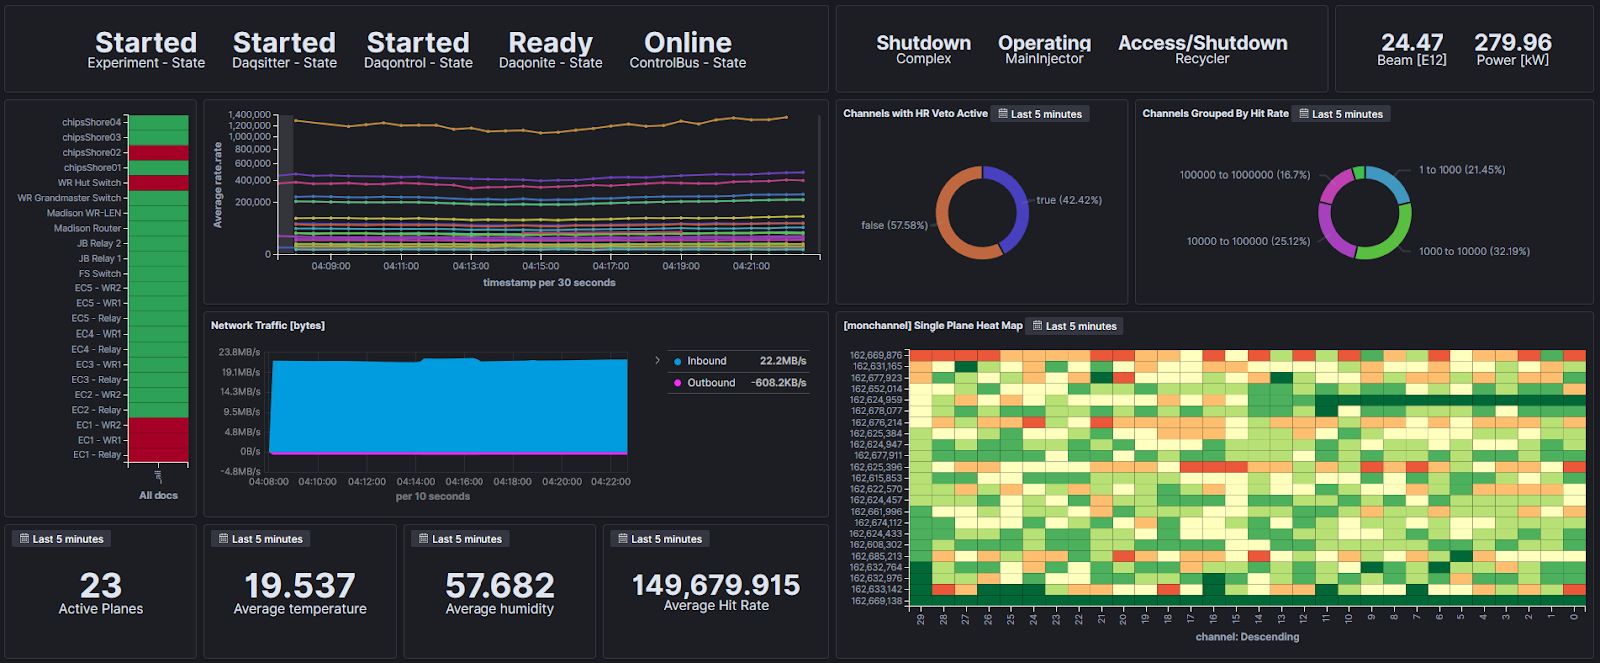
\includegraphics[width=0.8\textwidth]{diagrams/5-daq/monitoring.png}
    \caption[monitoring short]{monitoring long}
    \label{fig:monitoring}
\end{figure}
- Spill server diagram, probably combined with another diagram
- WR Switch
\begin{figure}
    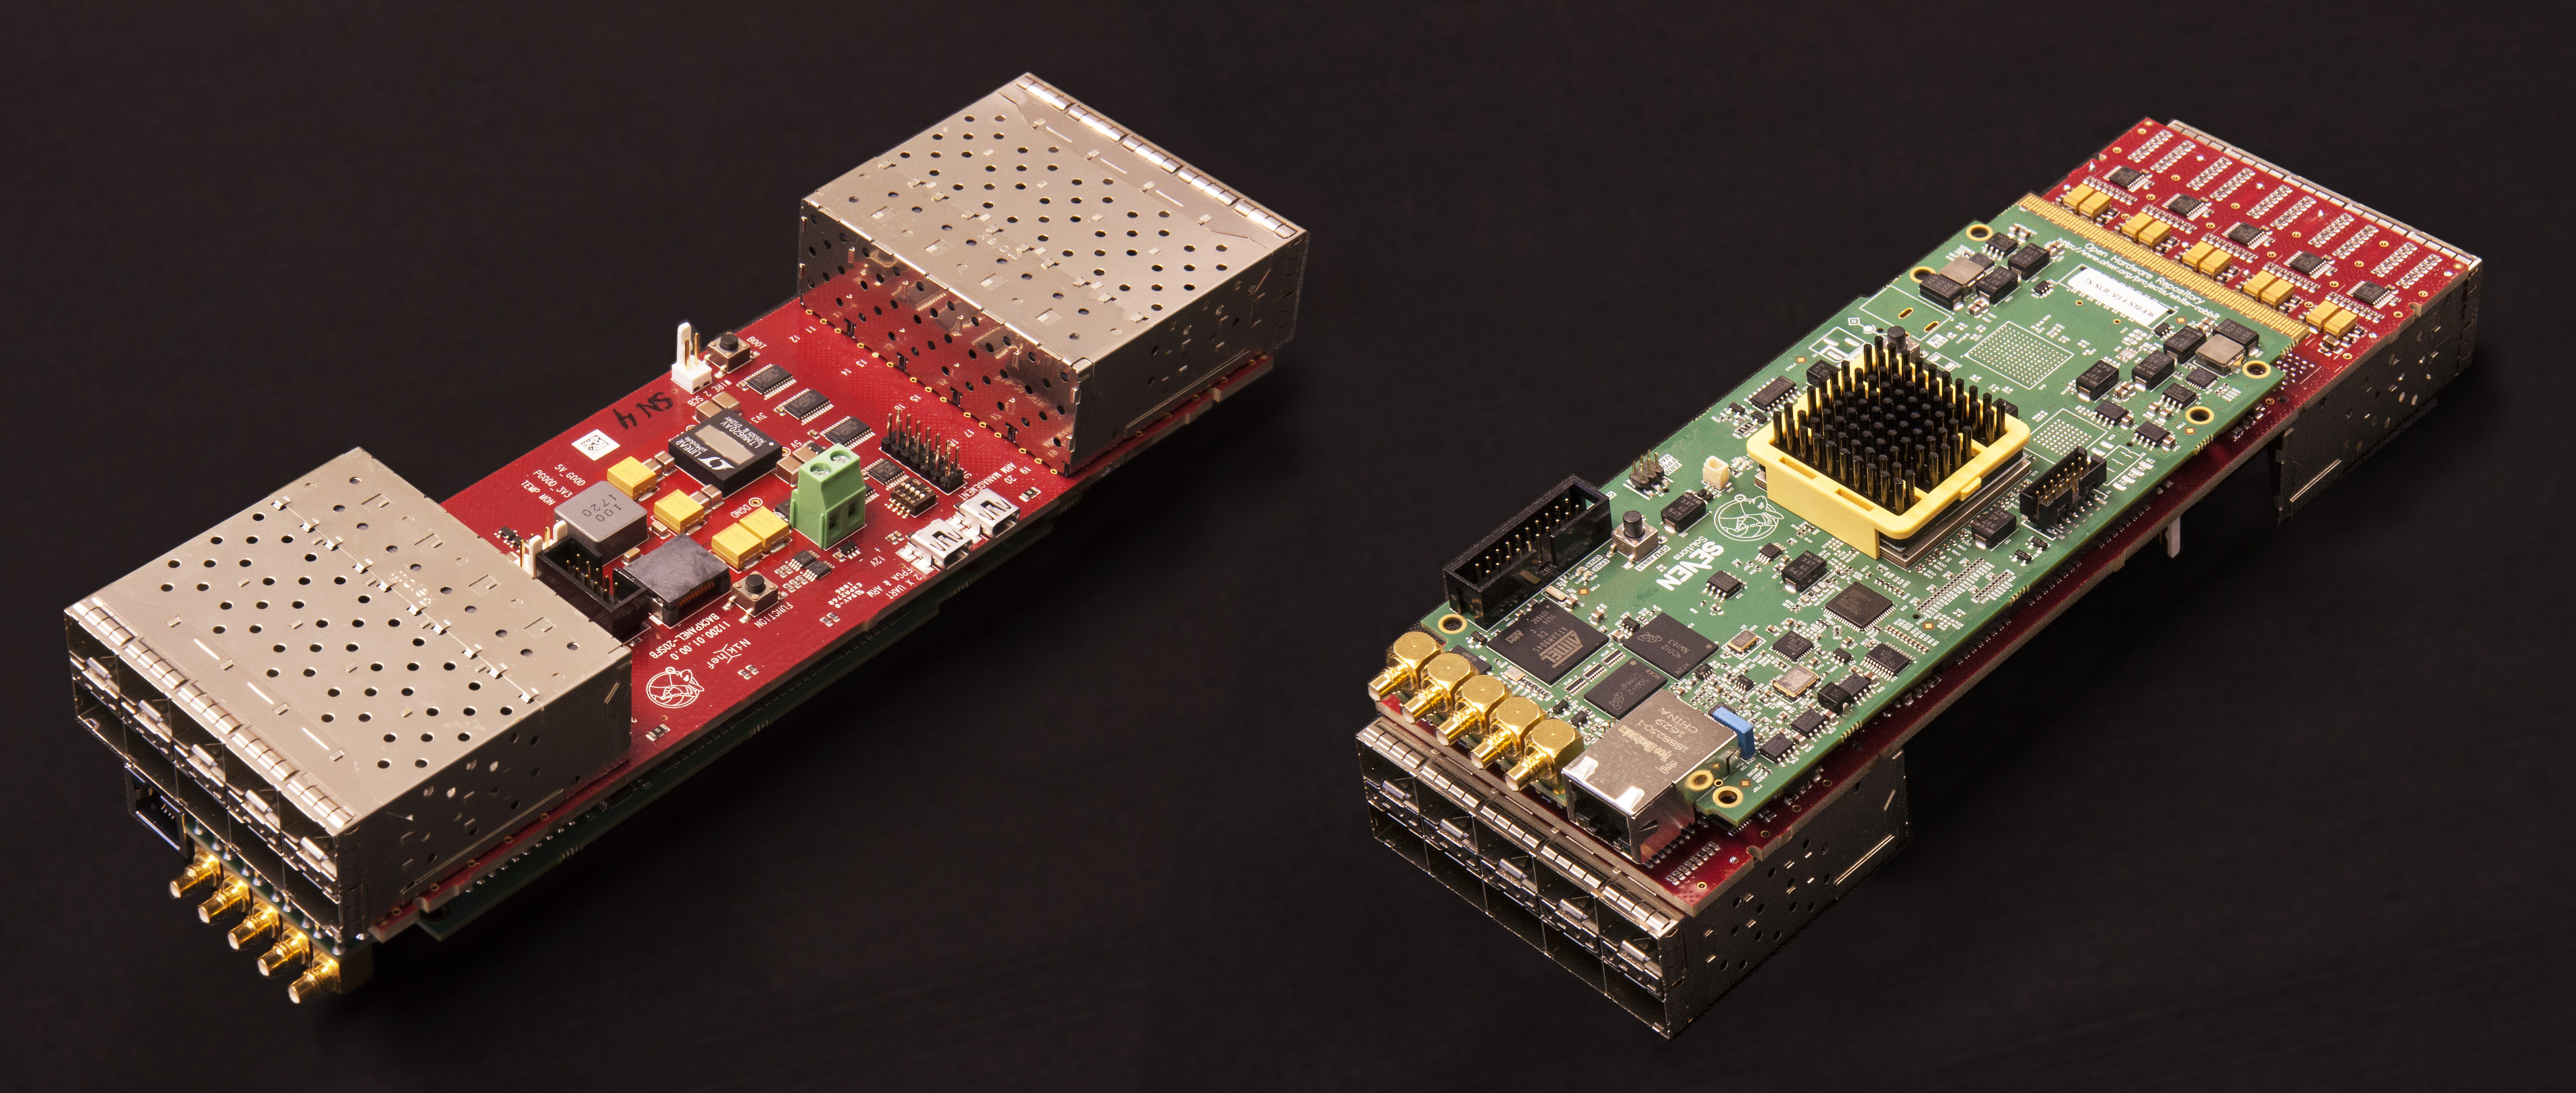
\includegraphics[width=0.8\textwidth]{diagrams/5-daq/wr_switch.jpg}
    \caption[wr switch short]{wr switch long}
    \label{fig:wr_switch}
\end{figure}
- WR GM Hut
\begin{figure}
    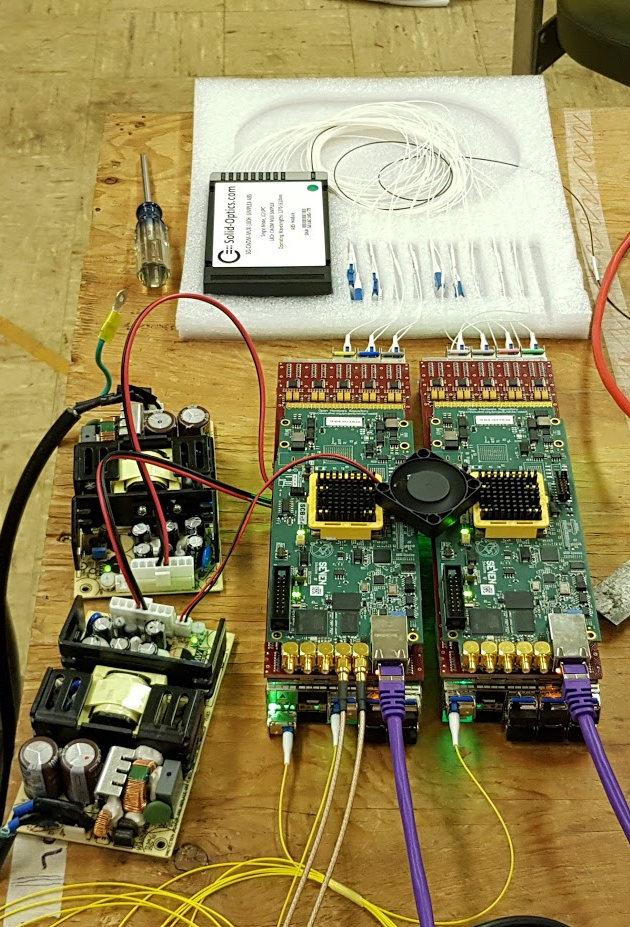
\includegraphics[width=0.8\textwidth]{diagrams/5-daq/wr_gm.jpg}
    \caption[wr gm short]{wr gm long}
    \label{fig:wr_gm}
\end{figure}
- WR LEN
\begin{figure}
    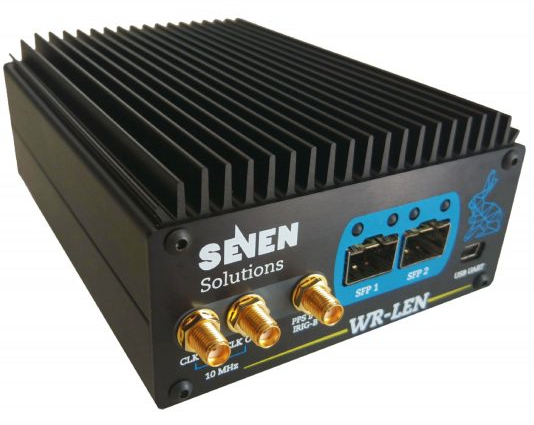
\includegraphics[width=0.8\textwidth]{diagrams/5-daq/wr_len.jpg}
    \caption[wr len short]{wr len long}
    \label{fig:wr_len}
\end{figure}
- Switch sync photo
\begin{figure}
    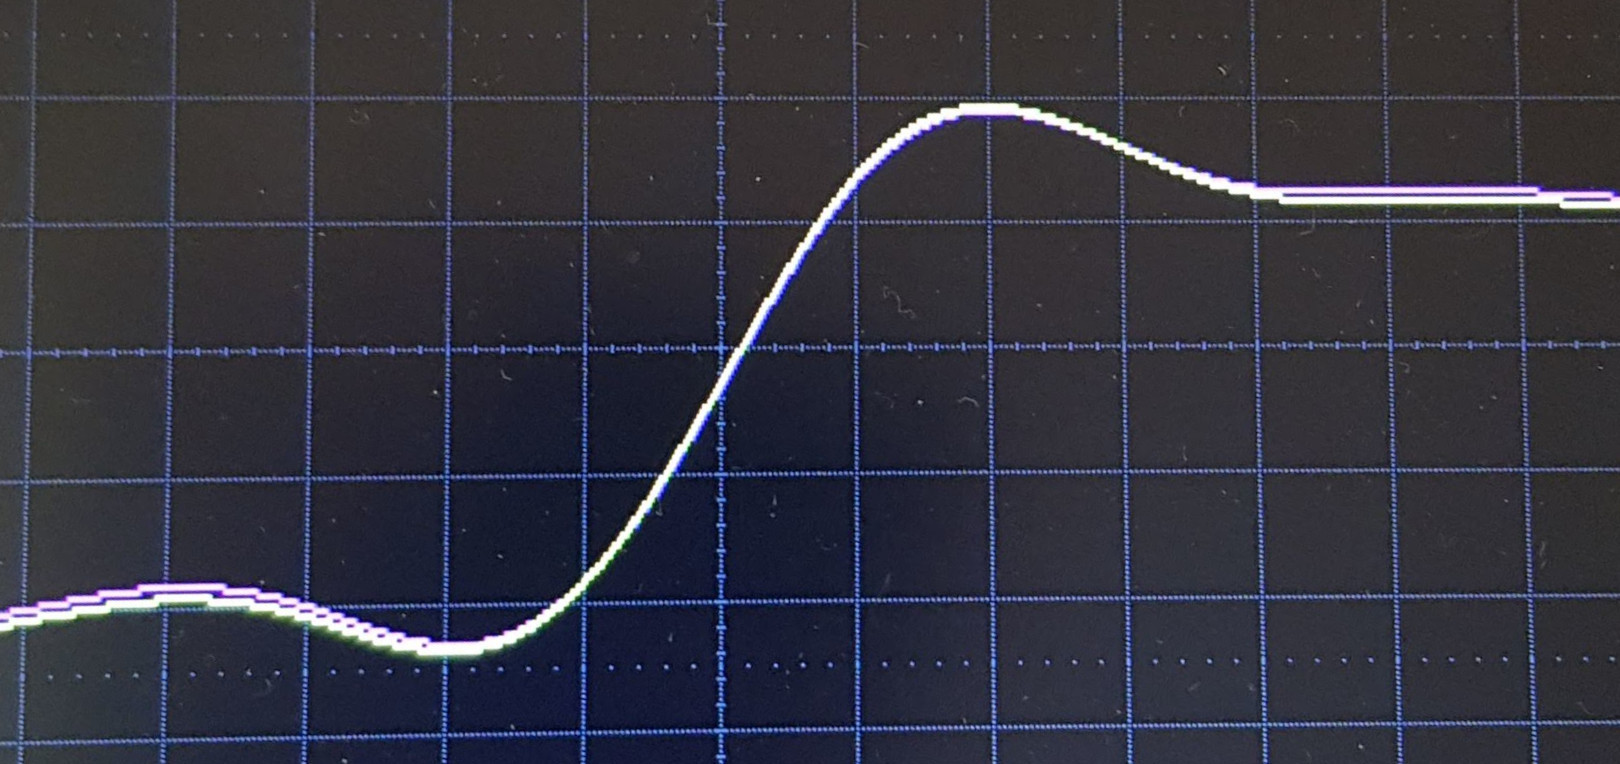
\includegraphics[width=0.8\textwidth]{diagrams/5-daq/sync.jpg}
    \caption[sync short]{sync long}
    \label{fig:sync}
\end{figure}
- Nikhef PMT
\begin{figure}
    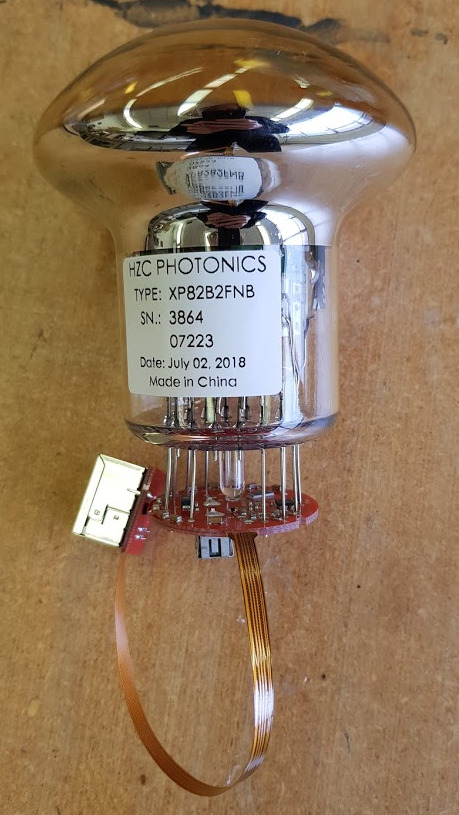
\includegraphics[width=0.8\textwidth]{diagrams/5-daq/nikhef_pmt.jpg}
    \caption[nikhef pmt short]{nikhef pmt long}
    \label{fig:nikhef_pmt}
\end{figure}
- CLB with wires
\begin{figure}
    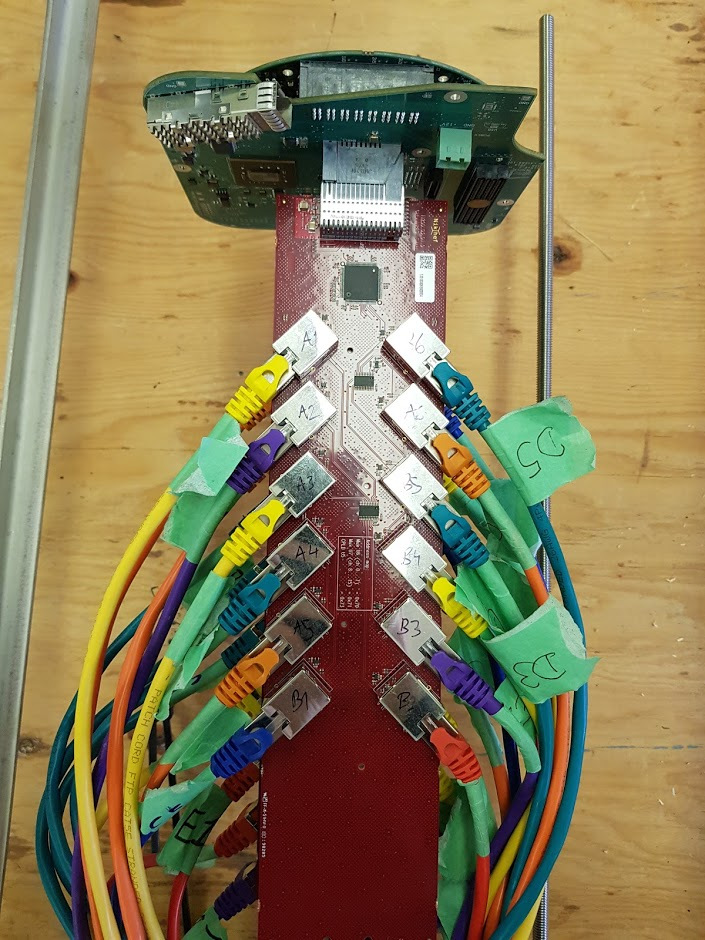
\includegraphics[width=0.8\textwidth]{diagrams/5-daq/clb.jpg}
    \caption[clb short]{clb long}
    \label{fig:clb}
\end{figure}
- CLB Rockets
\begin{figure}
    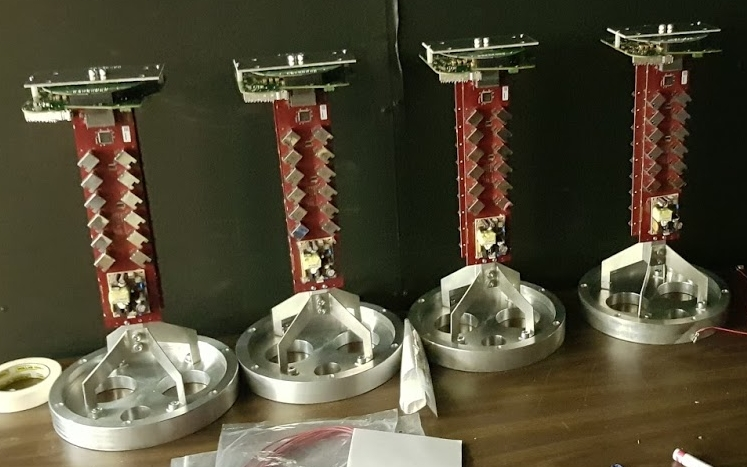
\includegraphics[width=0.8\textwidth]{diagrams/5-daq/rockets.jpg}
    \caption[rockets short]{rockets long}
    \label{fig:rockets}
\end{figure}
- Single plane
\begin{figure}
    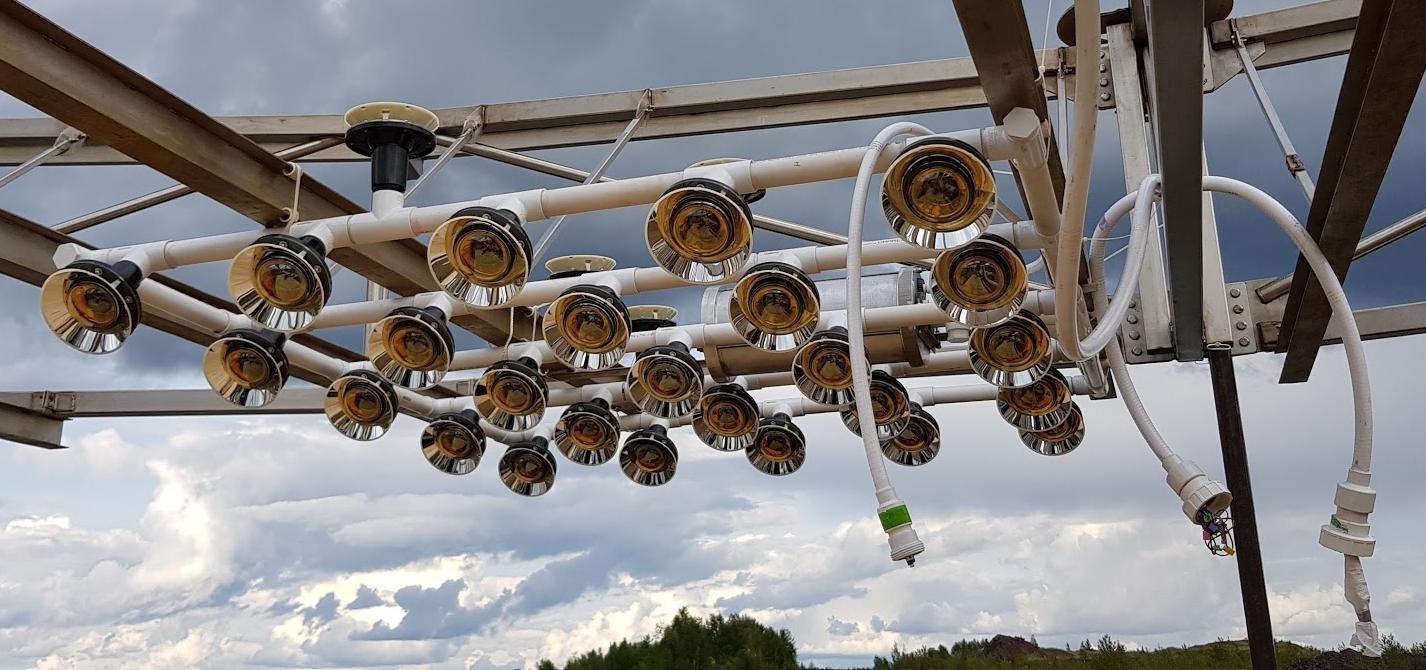
\includegraphics[width=0.8\textwidth]{diagrams/5-daq/single_plane.jpg}
    \caption[single plane short]{single plane long}
    \label{fig:single_plane}
\end{figure}
- TOT diagram
\begin{figure}
    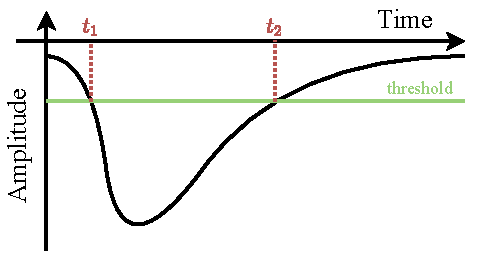
\includegraphics[width=0.8\textwidth]{diagrams/5-daq/tot.pdf}
    \caption[tot short]{tot long}
    \label{fig:tot}
\end{figure}
- Badger board with beaglebone picture
\begin{figure}
    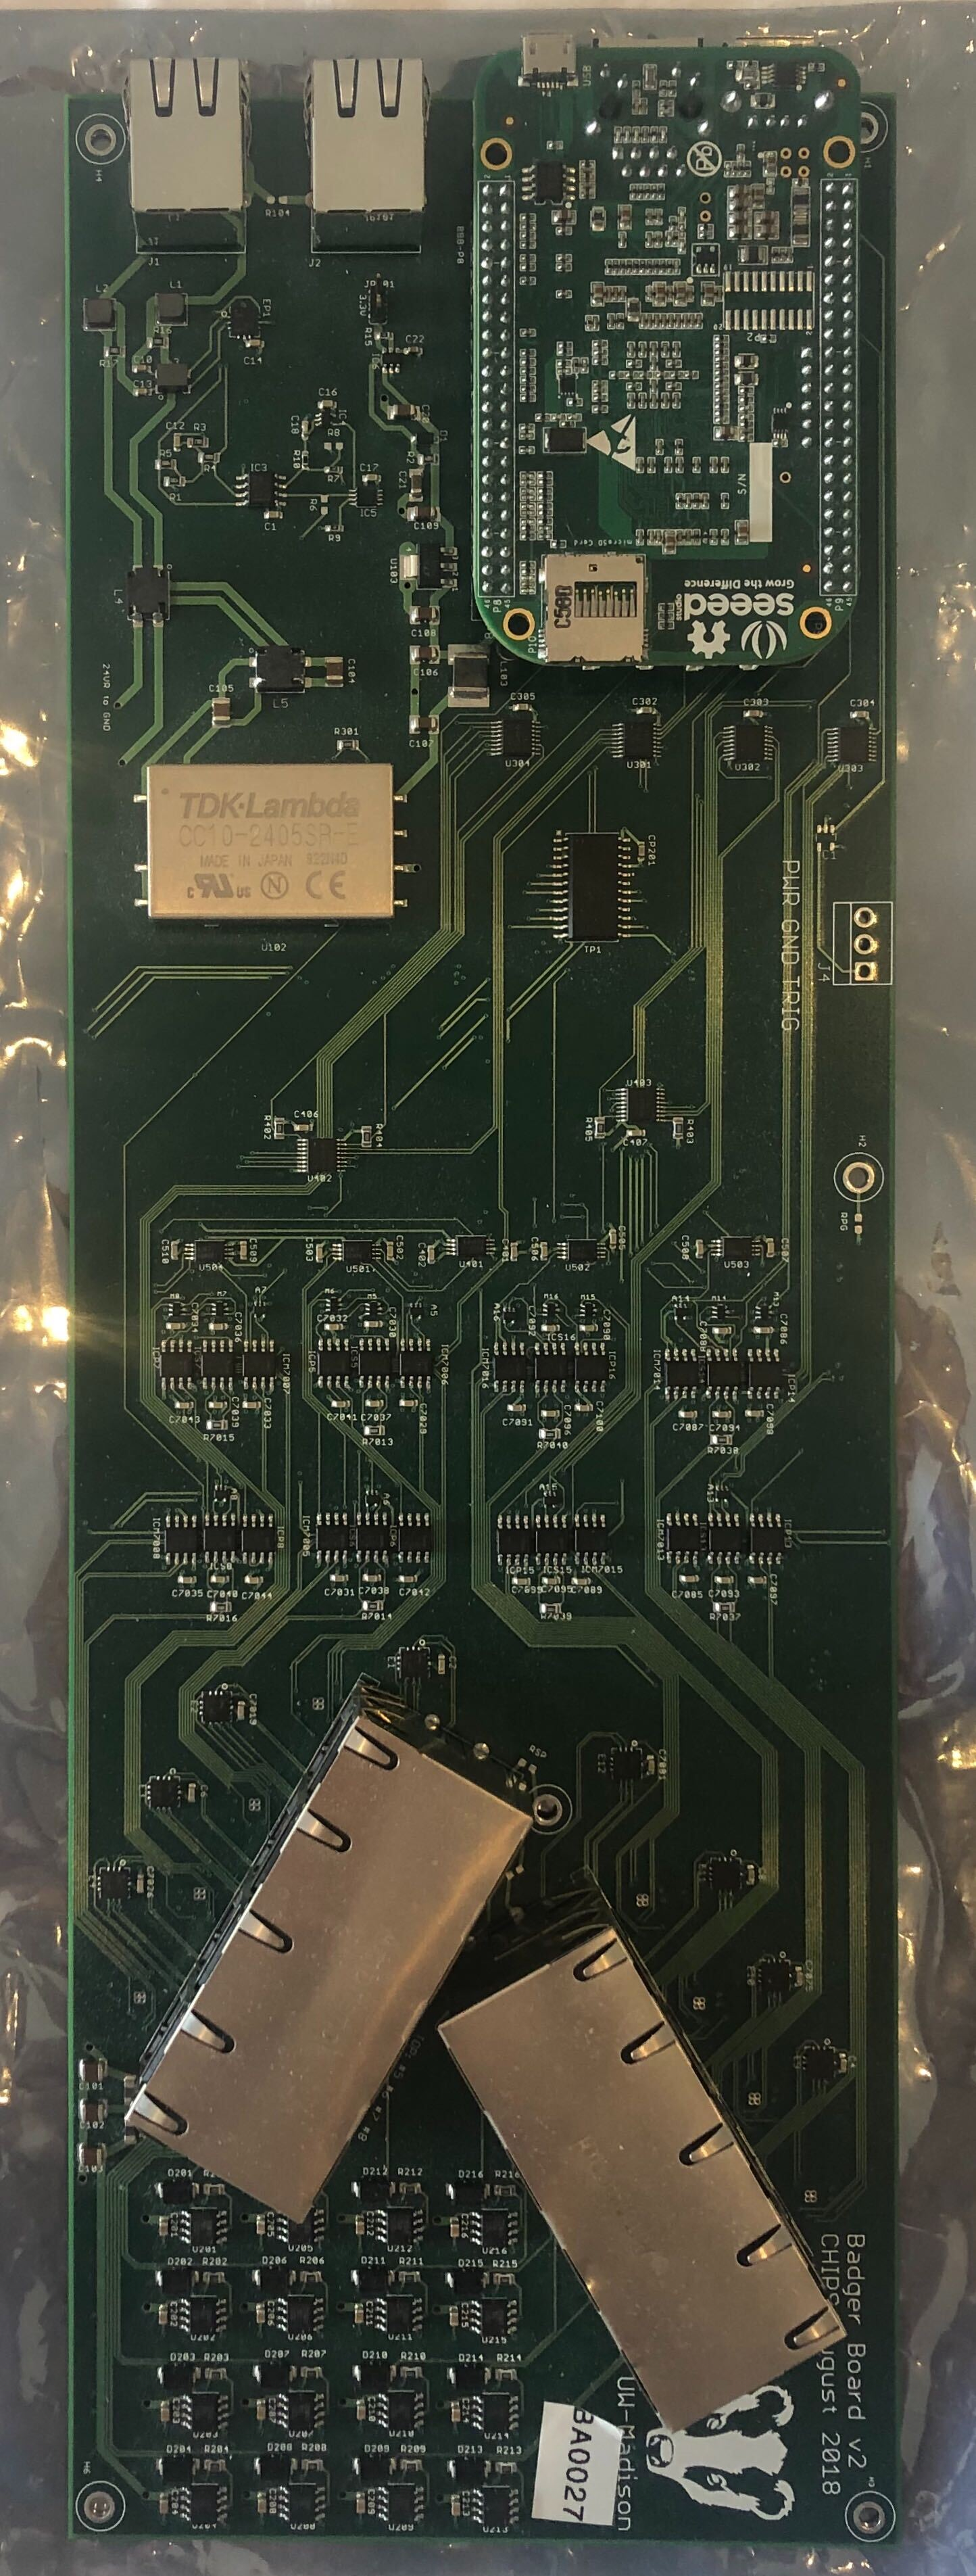
\includegraphics[angle=90,origin=c,width=0.8\textwidth]{diagrams/5-daq/badger.jpg}
    \caption[badger short]{badger long}
    \label{fig:badger}
\end{figure}
- Beaglebone picture
\begin{figure}
    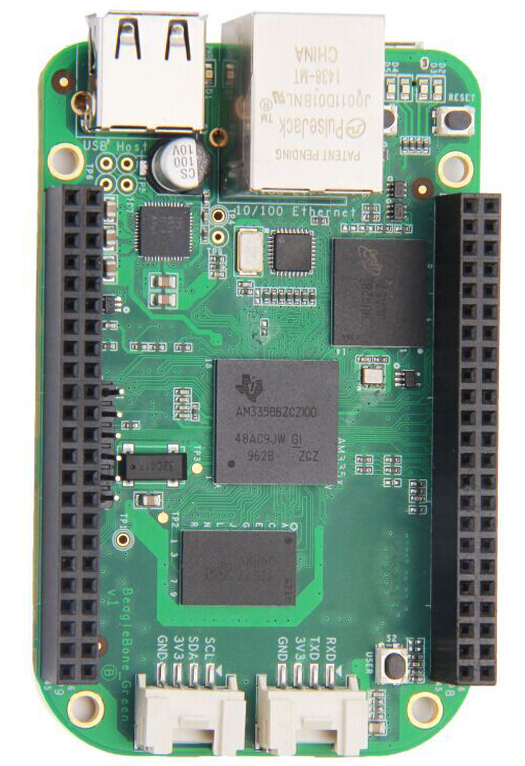
\includegraphics[width=0.8\textwidth]{diagrams/5-daq/beaglebone.jpg}
    \caption[beaglebone short]{beaglebone long}
    \label{fig:beaglebone}
\end{figure}
- Danout picture
\begin{figure}
    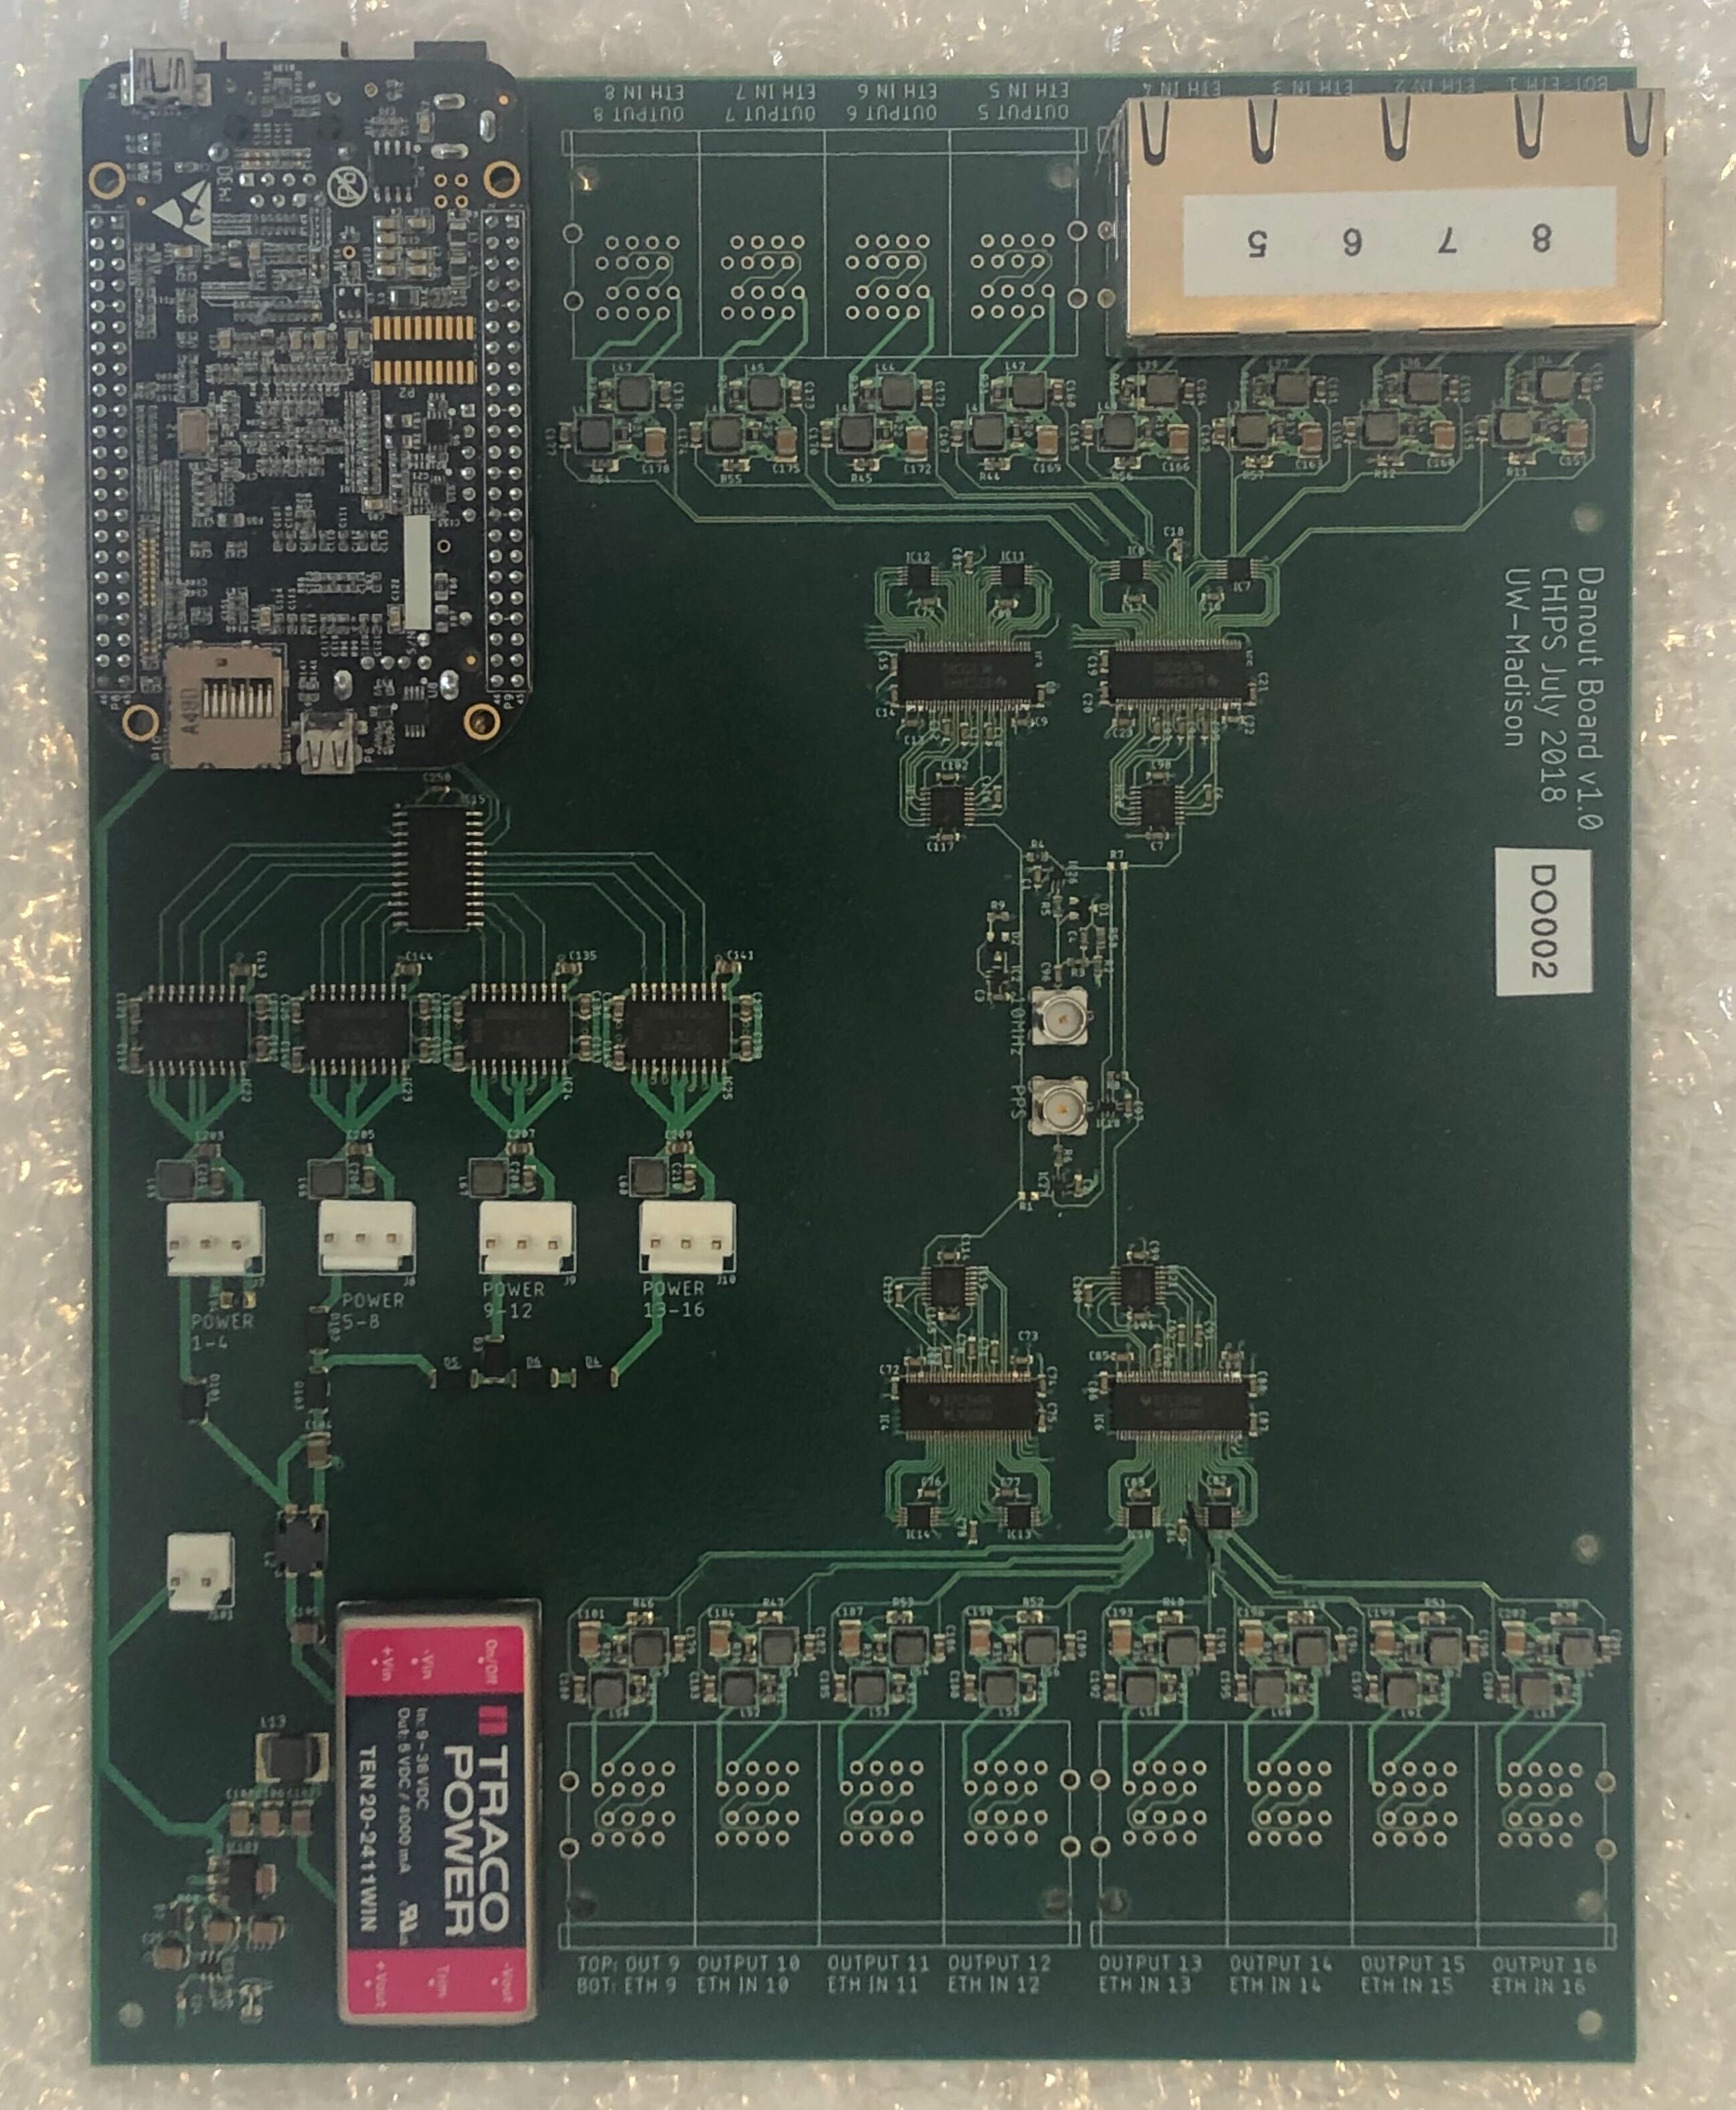
\includegraphics[angle=90,origin=c,width=0.8\textwidth]{diagrams/5-daq/danout.jpg}
    \caption[danout short]{danout long}
    \label{fig:danout}
\end{figure}

\section{References}

- WR Papers
- km3net daq Papers
- PMT time resolution Papers

\section{Reference notes}